\section{Implementation}
Game Mechanics function as basic systems of a game that governs their respective game elements (\cite{adams2012game}). All possible basic functions(represented by algorithms and data structures) and rules in the game are part of the mechanics. The section will discuss about planned game mechanics and their implementation.

\subsection{Web application}
The game will be a web application, this is because web applications are easily accessible and can be played on any device with a web browser. The game will be built using Angular as its frontend, a popular web application frontend framework and Flask as its backend, as it is a python lightweight backend compared to its alternatives. The UI was developed with PixiJS, A HTML5 creation engine that renders 2D graphics. There was no generic game engine used.

As central storing database, MongoDB was used. This is because MongoDB is a NoSQL database, which is a good choice for storing JSON data and long strings of user code. This database's main purpose is to stores all relevant information regarding the game content and will contain possible analytics in the future. It's base entity is the "Users" entity as shown in Figure \ref{fig:users}. Upon the creation of a "Users" entity, all other relating entities with references should also be created.
\begin{figure}[h]
    \centering
    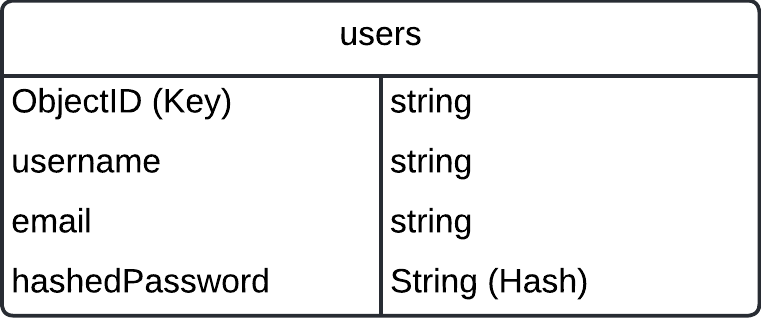
\includegraphics[width=0.5\linewidth]{images/user_object.png}
    \caption{Database model of the \textit{Users} entity}    
    \label{fig:users}
\end{figure}

\subsection{Level selection}
The game will have multiple levels, each level will have a different set of challenges. The player will have to complete each level to progress to the next. The levels will be designed to increase in difficulty as to teach the player different concepts of Python programming.

In the initial level selection, the player will be presented with a list of levels. Each level will have a title, a description, and a button to start the level. The player will be able to see the buttons of the levels they cannot access disabled and greyed out until they have completed the previous level. This is kept track by the leaderboard, which will be discussed in the next section.

\subsection{Leaderboard}
According to \cite{https://doi.org/10.1111/jcal.13077}, different designs of leaderboards can maximise either performance, motivation or engagement. Lower ranking students should be anonymised to prevent demotivation, and an absolute real leaderboard which shows the points & ranking of the students should also be in place to encourage competition. Figure \ref{fig:leaderboard} shows the final design of the leaderboard decided on.

\begin{figure}[H]
    \centering
    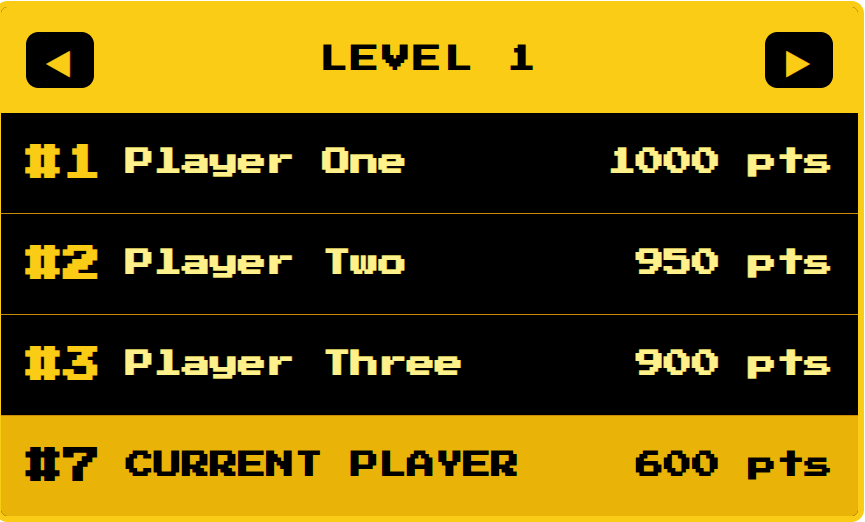
\includegraphics[width=0.5\linewidth]{images/leaderboard.png}
    \caption{Leaderboard design}    
    \label{fig:leaderboard}
\end{figure}

The leaderboard will store each player's data in the form of an entity in the database as shown in Figure \ref{fig:leaderboard_object}
\begin{center} 
    \begin{figure}[H]
        \centering
        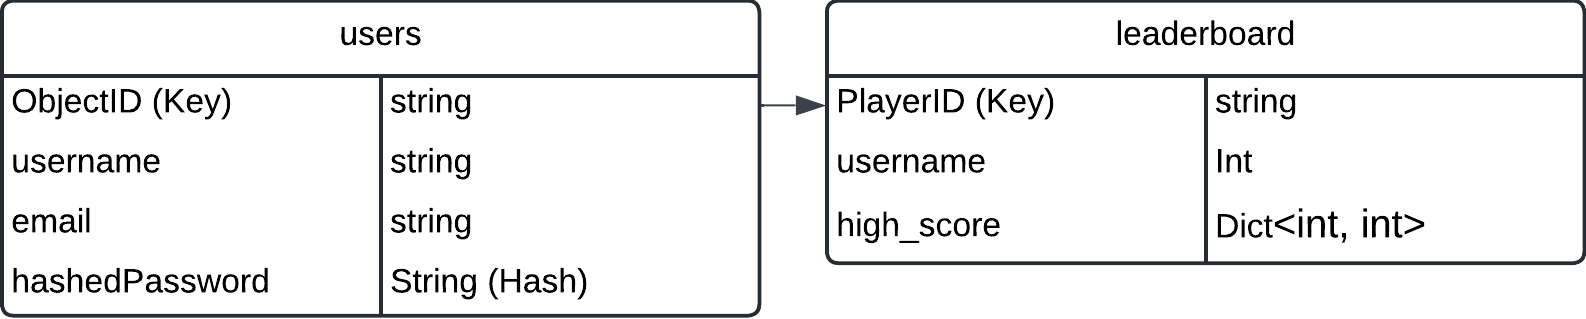
\includegraphics[width=0.5\linewidth]{images/leaderboard_object.png}
        \caption{Database model of the \textit{Leaderboard} entity}    
        \label{fig:leaderboard_object}
    \end{figure}
\end{center}
The backend will have an endpoint to handle the leaderboard, this endpoint will have basic CRUD functionality for the following basic use cases:
\\\\
% It will also handle data validation and edge cases in a following manner:
\begin{table}[H]
    \caption{Basic use cases}
    \begin{tabular}{|p{11cm}|p{5cm}|}
        \hline
        Use Case & Basic path\\
        \hline
        Player has completed a level and has a valid matching "User" entity & Add the player to the database\\
        \hline
        Player wants to view the leaderboard & Read the database\\
        \hline
        Player completes a level & Update the leaderboard\\
        \hline
        Player has a new high score & Update the leaderboard\\
        \hline
        Player has completed a level but does not have a valid matching "User" entity & Return an error\\
        \hline
    \end{tabular}
\end{table}

\subsection{Achievements}
\begin{wrapfigure}{r}{0.5\textwidth}
    \centering
    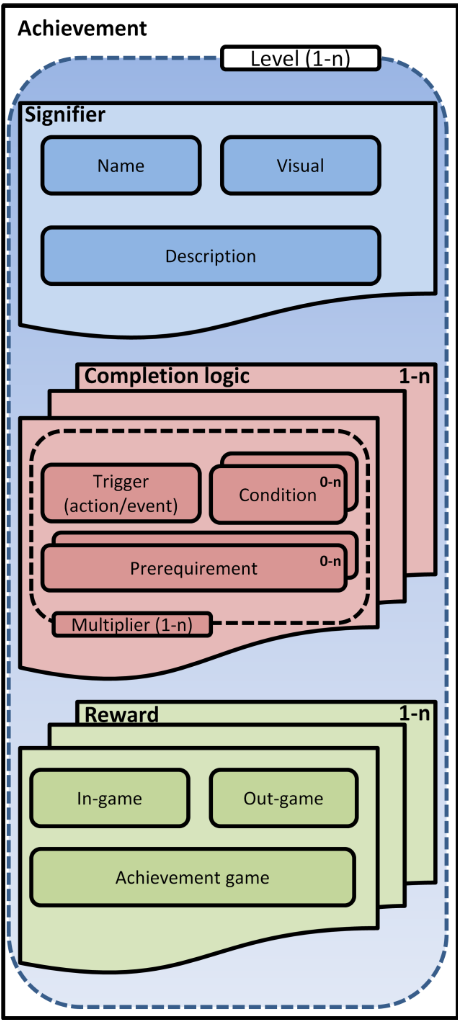
\includegraphics[width=0.5\linewidth]{images/achievement_framework.png}
    \caption{Achievement Framework\cite{hamari2011framework}}
\end{wrapfigure}
According to \cite{hamari2011framework}, achievements are composed mainly of a signifier, completion logic, and a reward. The Signifier element consists of the visible parts of the achievement. The foundational logic of an achievement defines the trigger (a player-invoked action or a system-invoked event), how many times it has to be triggered,  under which conditions, and what pre-requirements exist. The Reward element defines the reward(s) a player acquires after unlocking the achievement, this can be as simple as a number going up.
\\\\
The signifier agreed upon for the project is in figure \ref{fig:achievements} that will be displayed on the achievements tab. The completion logic on each achievement will be different, but most achievements are planned to be achievable within the same level, hence there is no condition that is cross level and no need to store prerequirements in the database.
\begin{figure}[H]
    \centering
    
\includegraphics[width=0.5\linewidth]{images/example_achievement.png}
    \caption{Database model of the \textit{Achievements} entity}    
    \label{fig:achievements}
\end{figure}

For basic achievements to be stored, an achievement database schema has to be designed to fit with the player schema. Basic validation and verification also have to be implemented in the application layer to make sure no error occurs. This achievement db also has to serve basic CRUD functionality.


The game will have achievements that the player can unlock. Achievements will be unlocked by completing certain tasks in the game. The achievements will be stored in the database as shown in Figure \ref{fig:achievements_object}
\begin{figure}[H]
    \centering
    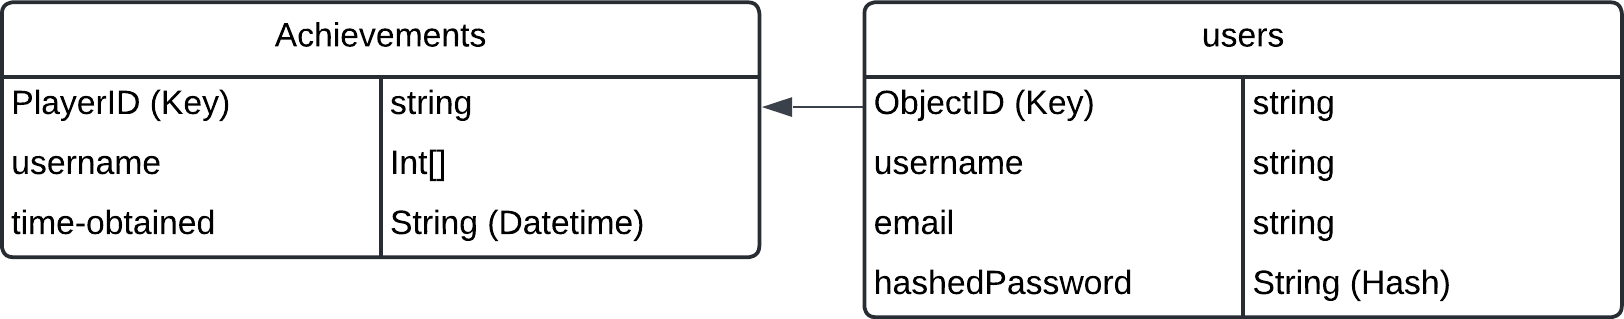
\includegraphics[width=0.5\linewidth]{images/achievements_object.png}
    \caption{Database model of the \textit{Achievements} entity}    
    \label{fig:achievements_object}
\end{figure}

\subsection{Code Input}
The whole user flow of the educational game, game flow\cite{kramarzewski2018practical}, can be simplified. It starts out with the user input, which would be the code submitted, the process would be the gameplay mechanics and the output would be the reward for the player.

This whole user experience starts with the user input, the submission of code can be done with a simple basic text box.
\begin{figure}[H]
    \centering
    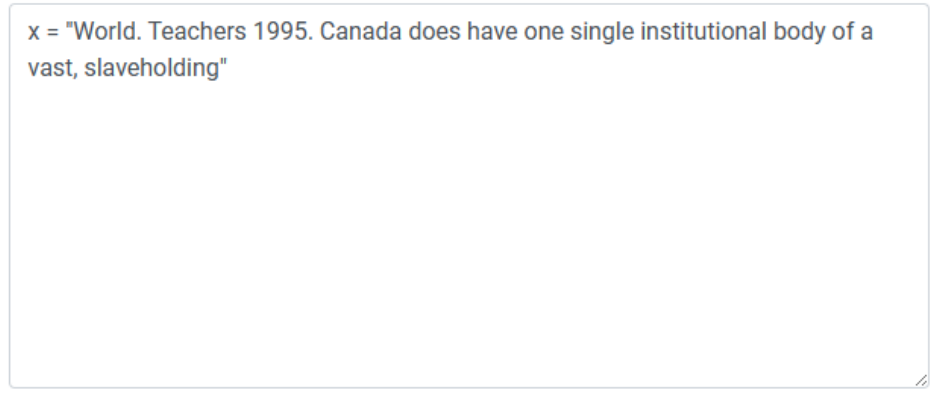
\includegraphics[width=0.5\linewidth]{images/textbox.png}
    \caption{Simple basic text box}
\end{figure}

To improve on this submission of code, we can use a code editor like professional integrated development environments (IDEs). An in-browser code editor such as Monaco or ace editor would suffice; additional improvements to build upon a code editor with other options such as night/day mode, a language server to verify Python syntax formatting, and other such Python language features as it is not natively implemented within editors such as Monaco. Other features that should be implemented to help with user experience would be code completion, syntax/semantic highlighter, definition provider, formatting provider, and more.
\\\\
\begin{figure}[H]
    \centering
    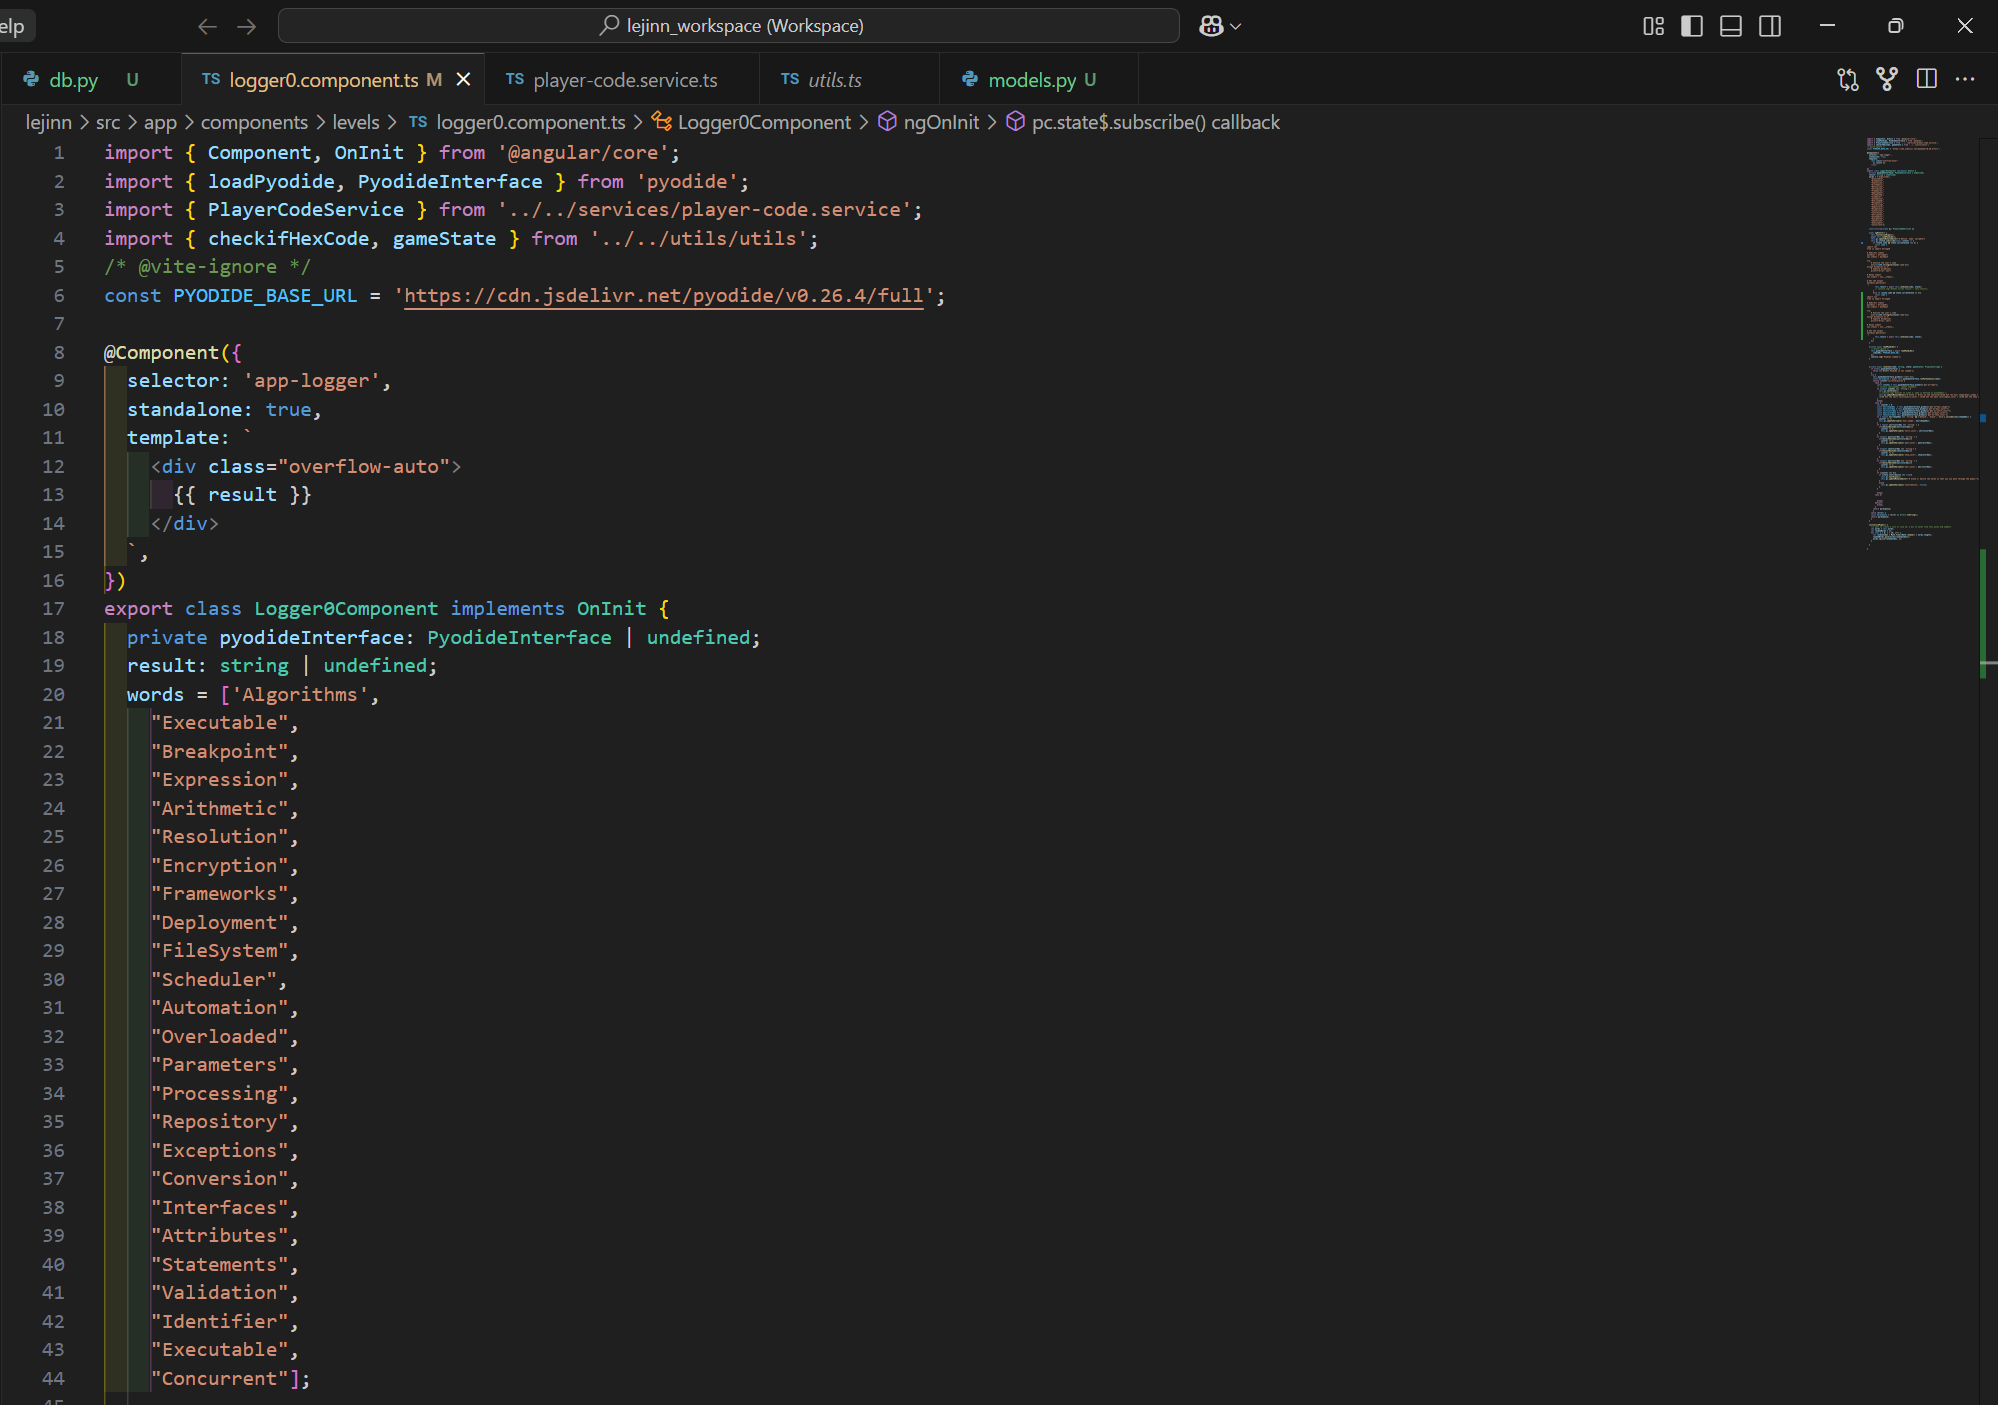
\includegraphics[width=0.3\linewidth]{images/code_editor.png}
    \caption{Code editor of IDE, a significant improvement over a basic textbox}
\end{figure}
Upon code submission, there is a reaction of the code that ran. This reaction of running code is usually known as standard output(stdout). This has to be printed out, including all results and any errors of the code. Other than just text printing with results of code submission, storytelling can take place here that is reactive upon successful results. 
